\documentclass[12pt, letterpaper, oneside, notitlepage, onecolumn]{article}
\author{William Baskin}
\title{Dynamic Festo Model}
\pagestyle{plain}

\usepackage{parskip}

\usepackage{textcomp}
\usepackage[utf8]{inputenc}
\usepackage[english]{babel}
\usepackage{listings}
\usepackage{color}
\usepackage{verbatim}
% \usepackage{soul}
\usepackage[margin=0.69in]{geometry}

% math
\usepackage{amsmath, amssymb, amsthm}
% \usepackage{amsmath, amssymb, amsthm, gensymb}

\usepackage{graphicx}
% \graphicspath{ {a1/e1/} }
% \includegraphics[height=6.75in,angle=270]{HW25}

\definecolor{dkgreen}{rgb}{0,0.6,0}
\definecolor{gray}{rgb}{0.5,0.5,0.5}
\definecolor{mauve}{rgb}{0.58,0,0.82}

\lstset{frame=tb,
  language=Python,
  aboveskip=3mm,
  belowskip=3mm,
  showstringspaces=false,
  columns=flexible,
  basicstyle={\small\ttfamily},
  numbers=none,
  numberstyle=\tiny\color{gray},
  keywordstyle=\color{blue},
  commentstyle=\color{dkgreen},
  stringstyle=\color{mauve},
  breaklines=true,
  breakatwhitespace=true,
  tabsize=3
}

\DeclareMathOperator*{\argmax}{arg\,max}

\DeclareMathOperator*{\argmin}{arg\,min}

\newcommand{\subsubsubsection}{\paragraph}
\newcommand{\bbs}[1]{\section{#1}}
\newcommand{\bbss}[1]{\subsection{#1}}
\newcommand{\bbsss}[1]{\subsubsection{#1}}
\newcommand{\bbssss}[1]{\subsubsubsection{#1}}

\newcommand{\norm}[1]{\left\lVert#1\right\rVert}

\usepackage[pdftex,
    pdfusetitle
    ]{hyperref}

\begin{document}
\maketitle

\section{General Model}

\subsection{$L_{angle}$}
\begin{equation}
l_{0} + l_{1} \cos{\left (\alpha + \theta_{des} \right )}
\end{equation}

\subsection{$k$}
\begin{equation}
\frac{1}{l_{rest}} \left(- l_{0} - l_{1} \cos{\left (\alpha + \theta_{des}
\right )} + l_{rest}\right)
\end{equation}

\subsection{$F$}
\begin{equation}
\frac{Torque_{des}}{d \cos{\left (\beta + \theta_{des} \right )}}
\end{equation}

\subsection{Pressure Model}
\begin{equation}
S a_{6} + \frac{Torque_{des} a_{5}}{d \cos{\left (\beta + \theta_{des} \right
)}} + a_{0} + a_{1} \tan{\left (a_{2} \left(a_{3} + \frac{- l_{0} - l_{1}
\cos{\left (\alpha + \theta_{des} \right )} + l_{rest}}{l_{rest}
\left(\frac{Torque_{des} a_{4}}{d \cos{\left (\beta + \theta_{des} \right )}} +
k_{max}\right)}\right) \right )}
\end{equation}

\subsection{Empirical Pressure Model (subs a*)}
\begin{equation}
15.6 S + \frac{1.23 Torque_{des}}{d \cos{\left (\beta + \theta_{des} \right )}}
- 192.0 \tan{\left (0.9342165 - \frac{2.0265 \left(- l_{0} - l_{1} \cos{\left
  (\alpha + \theta_{des} \right )} + l_{rest}\right)}{l_{rest} \left(-
  \frac{0.331 Torque_{des}}{d \cos{\left (\beta + \theta_{des} \right )}} +
  k_{max}\right)} \right )} + 254.3
  \end{equation}


\section{But What do I Linearlize?}

\subsection{Simplified Pressure Model}

In the static case, there should be minimal hysteresis or friction effects from
air filling, so the S term from the previous model will be disregarded for the
moment.

\begin{equation}
P = a_{0} + a_{1} * tan(a_{2} * (\dfrac{k}{a_{4} * F + k_{max}} + a_{3})) + a_{5} * F
\end{equation}

Collecting for F

\begin{equation}
\dfrac{P - a_{0}}{a_{1}} = tan(a_{2} * (\dfrac{k}{a_{4} * F + k_{max}} + a_{3})) +
\dfrac{a_{5}}{a_{1}} * F
\end{equation}

So, I don't think there's a neat and tidy way to solve for F. However, if my end
goal is to solve for torque and theta, then I could do a linear approximation to
estimate the spring-like properties. If I know the derivative of the pressure
function with respect to $\theta$ and $\tau$, then I can approximate the
relationship between the two for constant pressure near the approximation point
where the only two changing variables are assumed to be the joint angle and
torque.

\begin{equation}
P(\theta, \tau) \approx P(\theta^{*}, \tau^{*}) +
\dfrac{\partial P}{\partial \theta}(\theta^{*}, \tau^{*}) * (\theta -\theta^{*}) +
\dfrac{\partial P}{\partial \tau}(\theta^{*}, \tau^{*}) * (\tau - \tau^{*})
\end{equation}

In particular, the approximation point is the desired static point:

\begin{equation}
P(\theta, \tau) \approx P(\theta_{des}, \tau_{des}) + 
\dfrac{\partial P}{\partial \theta}(\theta_{des}, \tau_{des}) * (\theta -\theta_{des}) +
\dfrac{\partial P}{\partial \tau}(\theta_{des}, \tau_{des}) * (\tau - \tau_{des})
\end{equation}

\begin{equation}
P(\theta, \tau) \approx P(\theta_{des}, \tau_{des}) + 
\dfrac{\partial P}{\partial \theta}(\theta_{des}, \tau_{des}) * (e_{\theta}) +
\dfrac{\partial P}{\partial \tau}(\theta_{des}, \tau_{des}) * (e_{\tau})
\end{equation}

This approximates the joint behaving as a torsion spring for angles near the
desired angle, with a resting angle of 0 that corresponds to the desired angle.
If this is rearranged to move constant terms to the left:

\begin{equation}
P(\theta, \tau) - P(\theta_{des}, \tau_{des})
\approx
\dfrac{\partial P}{\partial \theta}(\theta_{des}, \tau_{des}) * e_{\theta}
+ \dfrac{\partial P}{\partial \tau}(\theta_{des}, \tau_{des}) * e_{\tau}
\end{equation}

The assumed current control sequence is that the controller maintains constant
pressure. Therefore, the constant controlled pressure $P(\theta, \tau) = 
P(\theta_{des}, \tau_{des})$. This simplifies the expression to the following:

\begin{equation}
0
\approx
\dfrac{\partial P}{\partial \theta}(\theta_{des}, \tau_{des}) * e_{\theta}
+ \dfrac{\partial P}{\partial \tau}(\theta_{des}, \tau_{des}) * e_{\tau}
\end{equation}

Solving for torque:

\begin{equation}
e_{\tau}
\approx
- \dfrac{\dfrac{\partial P}{\partial \theta}(\theta_{des}, \tau_{des})}{
\dfrac{\partial P}{\partial \tau}(\theta_{des}, \tau_{des})}
e_{\theta}
\end{equation}

This would indicate that the actuators behave like a torsion spring ($\Delta \tau =
-\kappa \Delta \theta$) for small changes in angle of the joint. The spring constant $\kappa$:

\begin{equation}
\kappa
=
- \dfrac{\dfrac{\partial P}{\partial \theta}(\theta_{des}, \tau_{des})}{
\dfrac{\partial P}{\partial \tau}(\theta_{des}, \tau_{des})}
\end{equation}

This means that the stability of the joint, for small angles near the desired
angle, approximates proportional control if constant pressure is maintained.

\section{Dual Actuator Model}

% TODO(buckbaskin): come back when I have a labeled model of how this fits
% together

\section{Dynamic Model}

From the paper "Modeling the Dynamic Characteristics of Pneumatic Muscle" by
Reynolds et. al. 2003, the pneumatic muscle can be modeled as the actuator, a
spring and a damper/dashpot. The above linearlized analysis is acceptable,
except that the linear system approximation there doesn't show any damping
effects, so the system's eigenvalues in linear analysis doesn't demonstrate the
expected stability.

\subsection{Proportional (In)Stability}

\begin{equation}
\begin{bmatrix}
\dot{x} \\
\ddot{x}
\end{bmatrix}
=
\begin{bmatrix}
0 & 1 \\
-K_{p} & 0
\end{bmatrix}
%
\begin{bmatrix}
x \\
\dot{x}
\end{bmatrix}
\end{equation}

\subsubsection{Eigenvalues}

The eigenvalues of the system as defined have a real component of 0 and
imaginary components. Therefore the system is unstable and oscillating with the
proportional linearized analysis.

\begin{center}
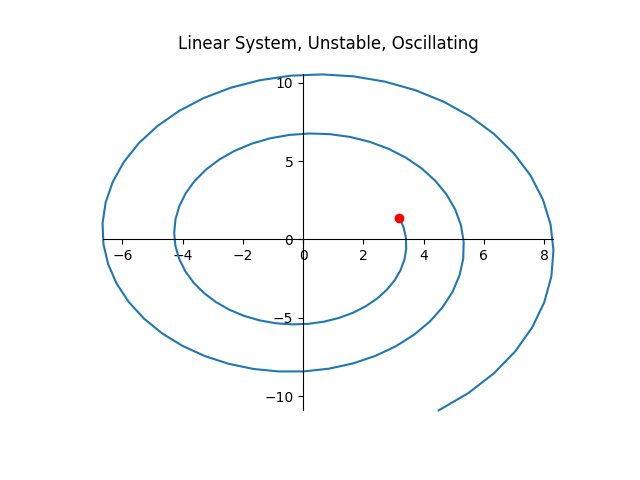
\includegraphics[width=3in,angle=0]{linear_unstable}
\end{center}

\subsection{PD Stability}

\begin{equation}
\begin{bmatrix}
\dot{x} \\
\ddot{x}
\end{bmatrix}
=
\begin{bmatrix}
0 & 1 \\
-K_{p} & -K_{v}
\end{bmatrix}
%
\begin{bmatrix}
x \\
\dot{x}
\end{bmatrix}
\end{equation}

\subsubsection{Eigenvalues}

The eigenvalues of the system as defined have a real component of 0 and
imaginary components. Therefore the system is unstable and oscillating with the
proportional linearized analysis.

For large $K_{v}$, the system is damped enough to be stable and converge.

\begin{center}
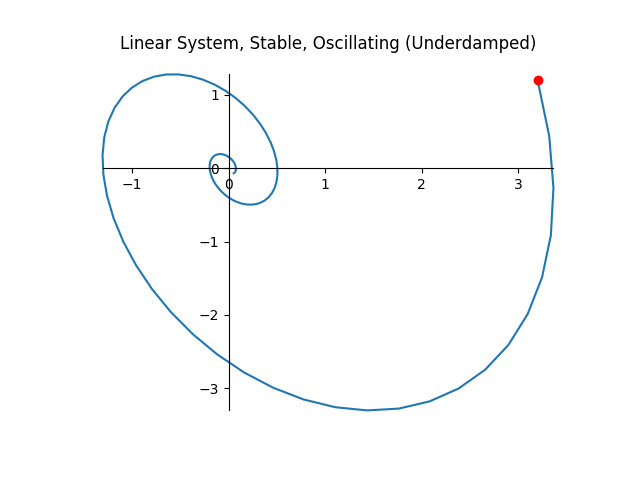
\includegraphics[width=3in,angle=0]{linear_pd_bigV}
\end{center}

For small $K_{v}$, the system is not damped enough to be stable and converge.

\begin{center}
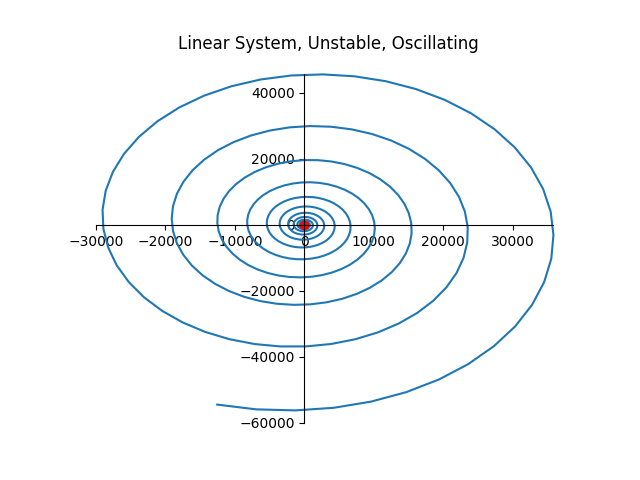
\includegraphics[width=3in,angle=0]{linear_pd_smallV}
\end{center}

For medium $K_{v}$, the system is damped just enough to be stable and
converge. For the example system, $K_{v} = 0.2$ the system oscillates back
through its starting point.

\begin{center}
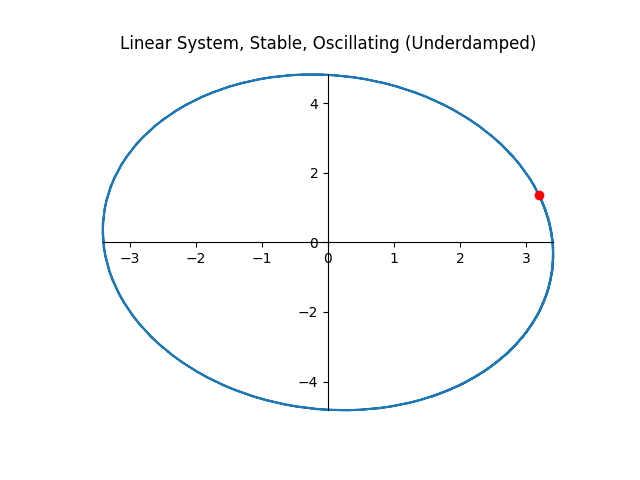
\includegraphics[width=3in,angle=0]{linear_pd_circleV}
\end{center}

For slightly larger $K_{v}$, the system is just damped enough to converge.

\begin{center}
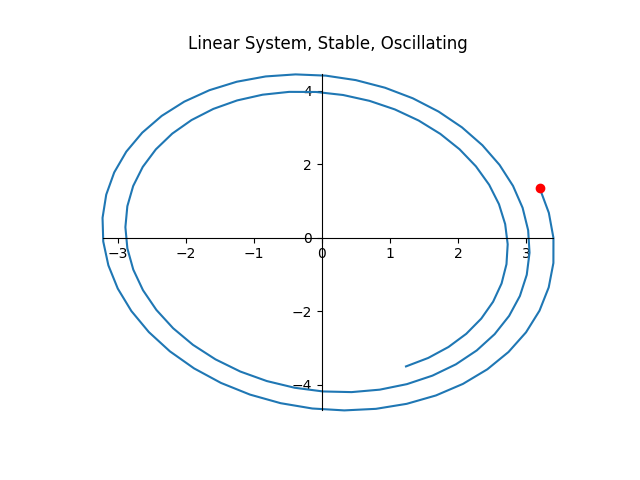
\includegraphics[width=3in,angle=0]{linear_pd_mediumV}
\end{center}

\subsubsection{Estimating $K_{v}$}

So, how does the $K_{v}$ for a pneumatic muscle compare? Based on the intuition
above, it can fit in one of many cases (stable/unstable, oscillating/not).

From Reynolds et. al. 2003, the damping increases with pressure on contraction
and decreases with pressure on relaxation. 

For a given pressure, one can linearize the change in $\dfrac{\partial
P}{\partial t}$ w.r.t. $\theta$ and $\tau$. The pressure is assumed to remain
constant, so the left side of the equation is assumed to be 0.

% TODO(buckbaskin): insert the equation

\end{document}
